\documentclass[main]{subfiles}
\begin{document}

%@@@@@@@@@@@@@@@@@@@@@@@@@@@@@@
% Main Topics: Edmond's Blossom algorithm, the Tutte-Berge formula
% Matching number in general graphs - 18.12.2017
% author: Vanessa Leite

\section{Matchings in general graphs}

\paragraph{Definition: a component of a graph is odd if it has an odd number of
vertices. For any graph $G$, let $\sigma(G)$ be the number of odd components of
$G$. For any graph $G=(V,E)$ and $U \subseteq V$, the graph obtained by
deleting all vertices in $U$ and all edges incident with $U$ is denoted by
$G \ U$.}

\paragraph{For a graph $G=(V,E)$, $v(G) = \displaystyle \min_{U \subseteq V}
\frac{1}{2}(|V| + |U| - \sigma(G - U))$.}

\paragraph{A graph $G=(V,E)$ has an perfect matching iff $G - U$ has at most
$|U|$ odd components for each $U \subseteq V$.}
\subparagraph{Proof:} Follows from previous formula, since $G$ has a perfect
matching iff $v(G) \geq \frac{1}{2} |V|$.

\paragraph{Let $G=(V,E)$ be a graph without isolated vertices. Then, $\rho(G) =
\displaystyle \max_{U \subseteq V} \frac{|U| + \sigma(G)}{2}$}

\subsection{Finding a maximum-cardinality matching}

\paragraph{The max-size algorithm in general graphs:}
The problem: we want to find an $M$-augmenting path.

\paragraph{jack Edmonds - 1965:} Every time that we find an odd cycle, we
shrink the graph by removing the cycle and adding a pseudonode at the cycle
place.

\paragraph{Definition of shrink} Let $X$,$Y$ be sets.
Shrink $Y$: $X/Y =
\begin{cases}
  X\text{, if } X \cap Y = \emptyset\\
  X \setminus Y \cup \{Y\} \text{where $\{Y\}$ is a super node} \\
\end{cases}$.

Let $G=(V,E)$ be a graph and $C \subseteq V$. $V/C$: replace all nodes in $C$
by a "super node" $C$.
For $e =\{u,v\} \in E$, then $e/C =
\begin{cases}
  \emptyset \text{, if } u \in C \text{ and } v \in C \\
  \{u,C\} \text{, if } v \in C, u \notin C \\
  \{u,v\} \text{, if } u,v \notin C\\
\end{cases}$\\
$E/C = \{ e/C: e \in E\}$ and $G/C = (V/C, E/C)$

\paragraph{Definition: Let $G=(V,E)$ and $M \subseteq E$. Let $W \subseteq V$
be all nodes missed by $M$. A \emph{walk} $(v_0, \dots, v_t)$ is called
$M$-alternating path if $\{v_i, v_{i+1}\}$ or $\{v_{i-1}, v_i\}$ belongs to
$M$ for $i \geq 1$.}

An $M$-alternating walk is called an $M$-blossom if $v_0, \dots, v_{t-1}$ are
all distinct and $v_0 = v_t \in W$, $t$ is odd.

\paragraph{Remark: an $M$-alternating walk from $v_0 \in W$ to $v_t \in W$ can
be found as follows:}
Let $D=(V,A)$. $A=\{(v,v^\prime): \exists x \in V$ st $\{v,x\} \in E$ and
$\{x,v^\prime\} \in M\}$. A directed path from $v_0$ to a node adjacent to
$v_t$ gives an $M$-alternating walk in $G$.

\paragraph{Matching algorithm $\mathcal{A}(M, G, W)$}

Parameters: $M$ matching, $G$ graph and $W$ missed nodes.

\begin{enumerate}
\item Find a shortest $W-W$-walk, i.e, from a missed node to another missed
node in $G$, $P$.
\item Check wether $P$ contains $M$-augmenting path
\subitem If yes, augment the path
\subitem Otherwise, construct $M$-blossom from $P$ with node set
$C \subseteq V$. Let $G = (V/C, E/C)$, $M^\prime = M/C$, $W^\prime$ are missed
nodes by $M^\prime$ in $G^\prime$. Call $\mathcal{A}(M^\prime, G^\prime,
W^\prime)$.
\end{enumerate}
If answer for $M^\prime$ is optimal, then $M$ is optimal.
If answer is a better matching, then expand it to a matching in G as indicated
in the next theorem.

\paragraph{Corollary: $v(G)$ can be computed in time $\mathcal{O}(\abs{V}^2
\abs{E})$ for an undirected graph}

\subparagraph{Proof:} Apply the above algorithm iteratively, starting with
$M = \emptyset$ until a maximum-size matching is attained. By using (10?), a
shortest M-alternating w-w-walk can be found in time $\mathcal{O}(|E|)$.
Moreover, the graph $G/C$ can be constructed in time $\mathcal{O}(|E|)$. Since
the recursion has depth at most $|V|$, each application of the algorithm above
takes $\mathcal{O}(|V||E|)$ time. Since the number of applications is at most
$|V|$, we have the time bound given.

\paragraph{Theorem: Let $C = (v_0, \dots, v_t)$ be an $M$-blossom. $M$ attains
$v(G) \iff M^\prime = M/C$ attains $v(G/C)$.}

\subparagraph{Proof:}
\begin{itemize}
\item "$\rightarrow$"
\subitem Let $P$ be $M$-augmenting path in $G$, wlog $P$ does not start in
$v_0$. $P \cap C = \emptyset$ is clear. $M$-augmenting path in $M$ will be on
$M^\prime$. Otherwise, $P = QR$, where $Q$ is the subpath in $P$ not visiting
any node in $C$, except the last node in $Q$. Replace last node in $Q$ by
supernode $C$. $C$ is missed by $M^\prime$ and therefore $Q/C$ is
$M^\prime$-augmenting path.
\item "$\leftarrow$"
\subitem Let $P^\prime$ be $M^\prime$-augmenting in $G^\prime = G/C$. If
$P^\prime$ does not use "super node" $C$, then $P^\prime$ is $M$-augmenting in
$G$. Otherwise, $P^\prime$ ends in the supernode $C$. Then, $\{u,C\}$ is in
$E^\prime(P^\prime)$. This corresponds to an edge in $E$ of the form
$\{u,v_i\}$.
\end{itemize}

\begin{figure}[!h]
  \centering
    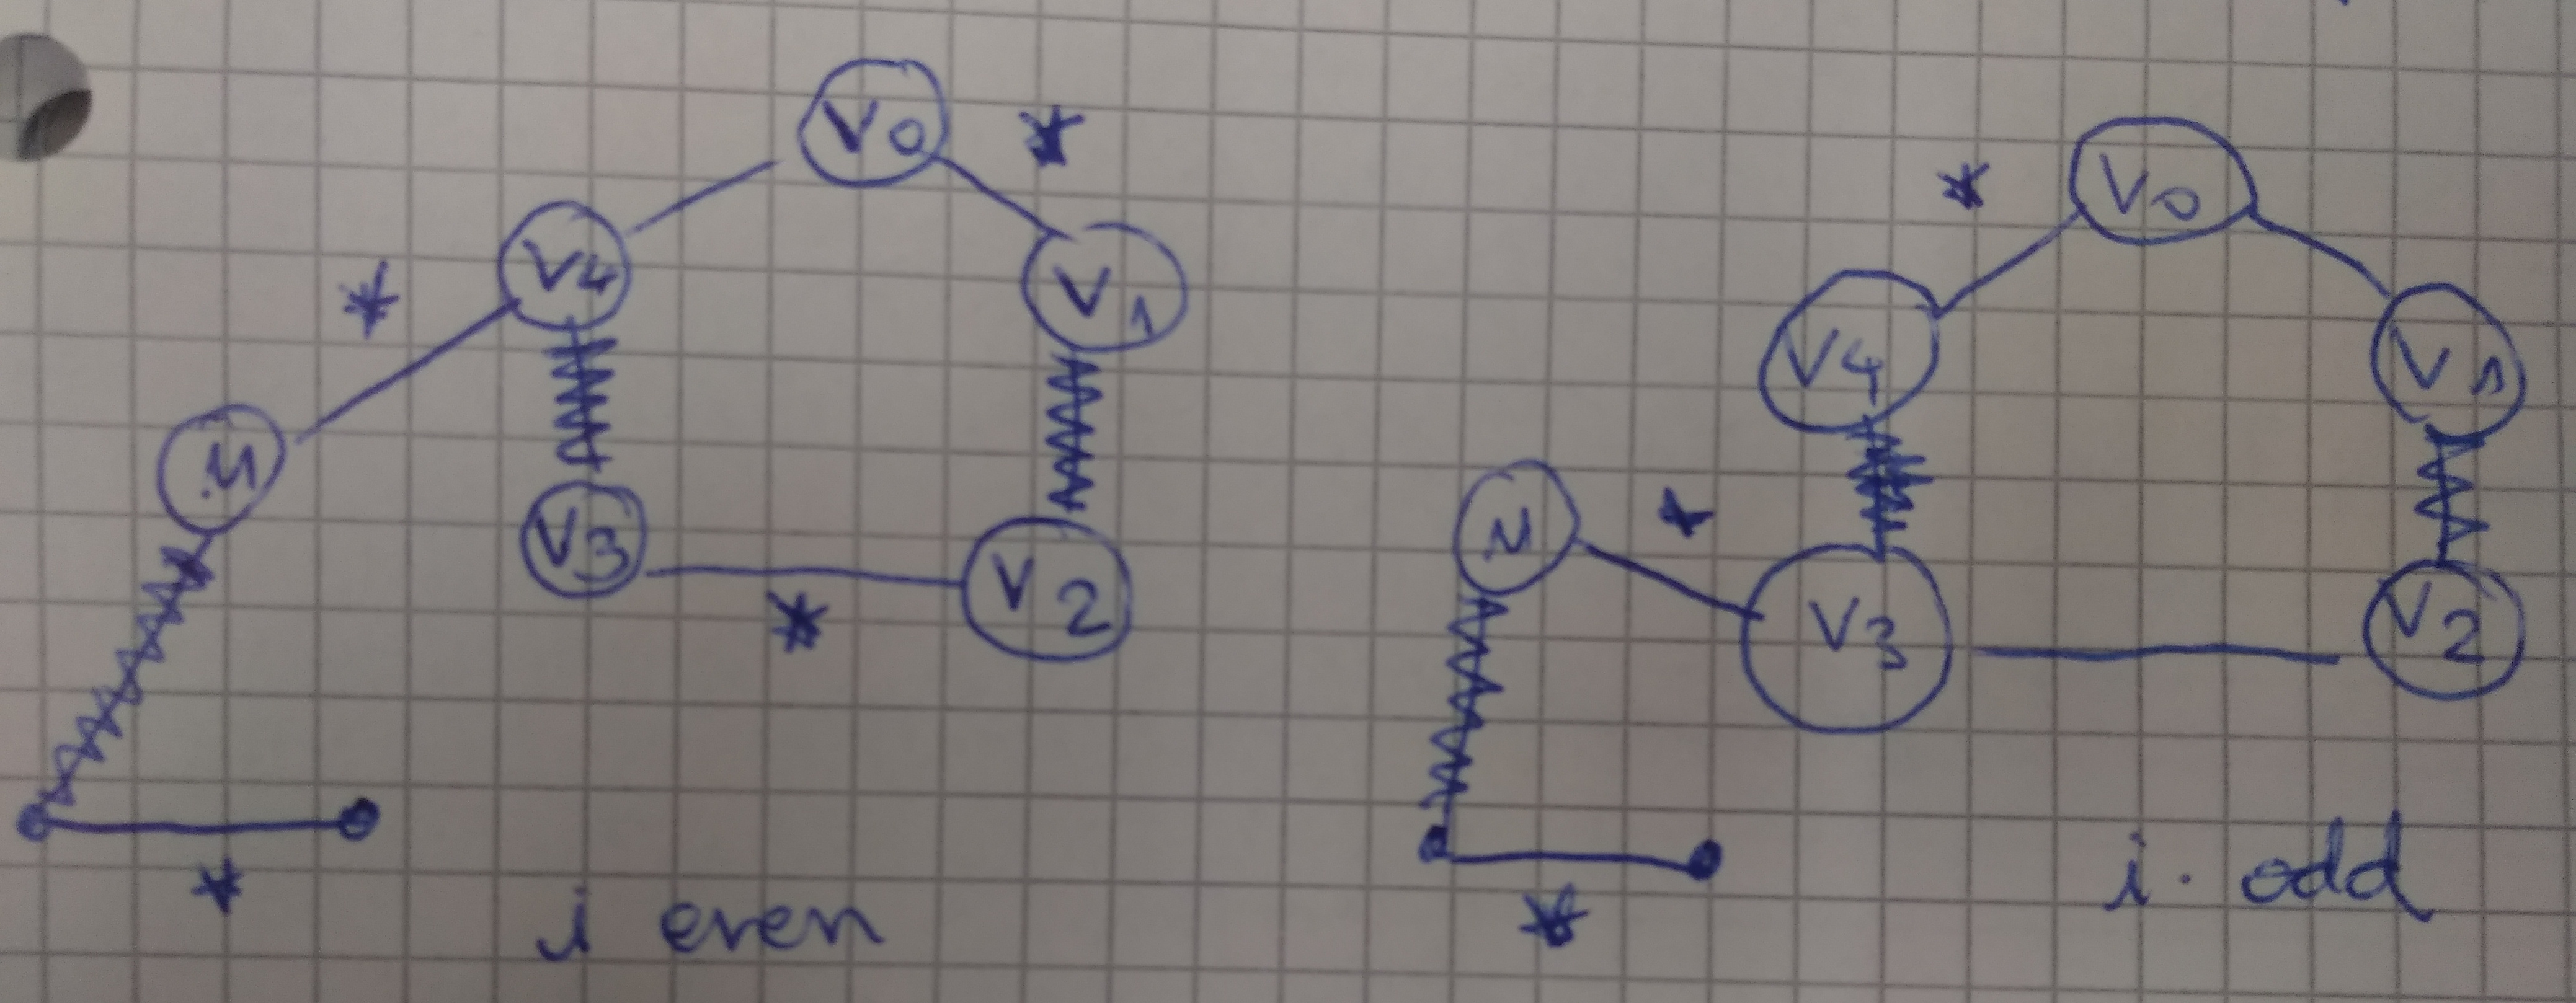
\includegraphics[width=0.3\textwidth]{imgs/supernode.jpg}
	\caption{If $i$ is even: replace supernode $C$ in $P$ by the sequence $v_i,
	v_{i-1}, \dots, v_0$. This gives $M$-augmenting path in $G$. If $i$ is odd:
	replace supernode $C$ in $P^\prime$ by the sequence $v_i, v_{i+1}, \dots,
	v_{t-1}, v_0$. This gives $M$-augmenting path in $G$.}
\end{figure}

\end{document}